% !TeX root = ./Serie03-JoelZuber-YannikDaellenbach.tex
% Suchen Sie zwei mobile Applikationen/Ansichten,
% wobei die erste Ansicht einen Signifier verwendet,
% der klar machen soll, dass der Benutzer nach rechts swipen kann 
% und die zweite Ansicht ohne Signifier hierfür klar kommt (also eine sichtbare Affordance besitzt). 
% Machen Sie Screenshots Ihrer Beispiele.
\begin{figure}[H]
  \centering
  \begin{minipage}[b]{0.45\textwidth}
    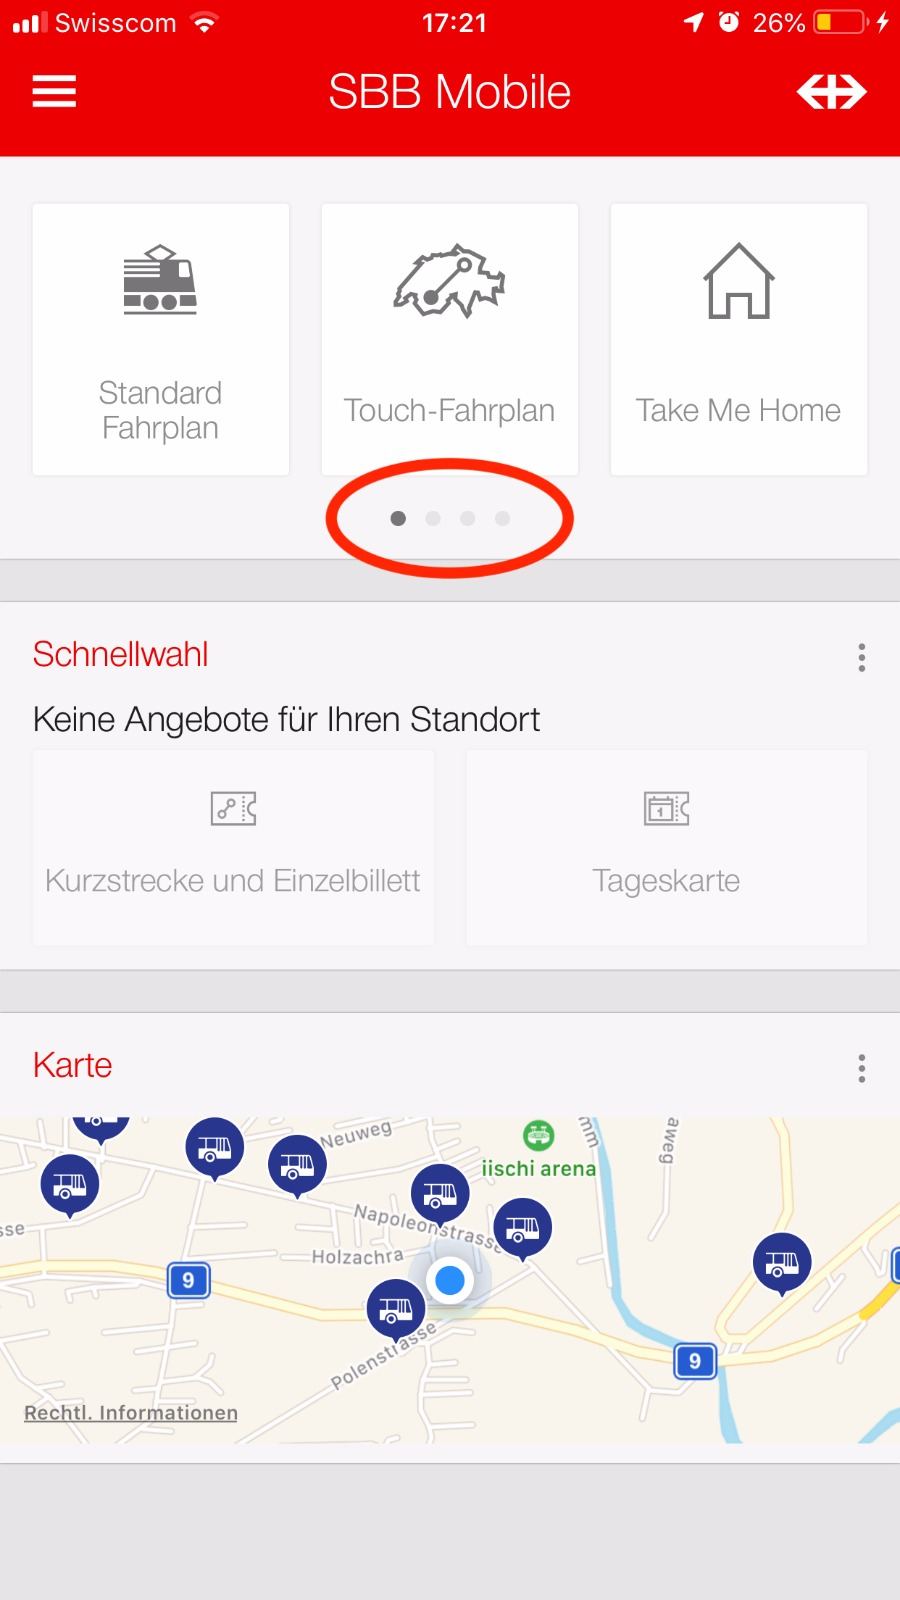
\includegraphics[width=\textwidth]{data/SBB.jpeg}  
    \label{fig:sbb}
    \caption{SBB Mobile}
  \end{minipage}
  \hfill
  \begin{minipage}[b]{0.45\textwidth}
    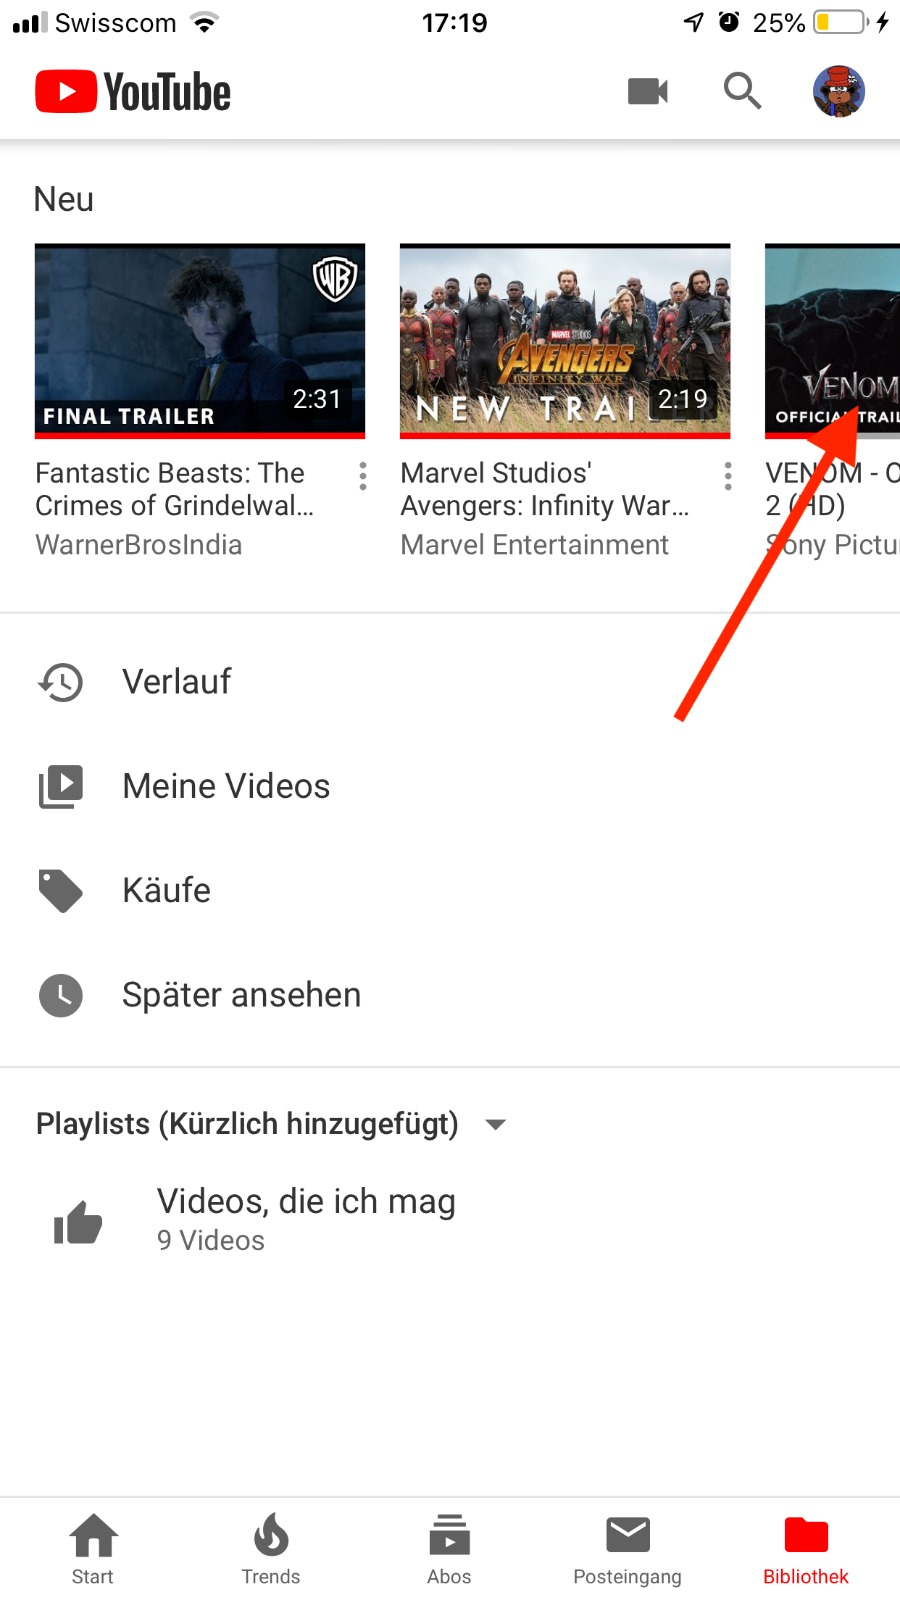
\includegraphics[width=\textwidth]{data/YouTube.jpeg}
    \caption{YouTube}
    \label{fig:youtube}
  \end{minipage}
\end{figure}

\subsection*{SBB Mobile}
Auf der Startseite der SBB Mobile App sind 
im ersten Abschnitt 3 Kacheln zu sehen und durch Swipen nach rechts erscheinen noch mehr. 
Hier dienen Punkte unter den Kacheln als Signifier.

\subsection*{YouTube}
In der Bibliothek-Ansicht der YouTube-App sieht man oben eine Liste neuer Videos. 
Es haben zwischen zwei und drei Vorschaubilder nebeneinander Platz, 
sodass das dritte Bild abgeschnitten ist. 
Somit ist auch ohne Signifier die Affordance erkennbar, 
dass durch Swipen nach rechts mehr Videos angezeigt werden können.
